
\startp
\upar{Определение температуры по потоку атомов}
Для определения температуры печи используется термопара, позволяющаю находить относительное изменение температуры, однако абсолютное значение $T_0$ было не откалибровано. Для калибровки термопары использовался следующий метод. Атомарный пучок, выходящий из печи, подсвечивался резонансным лазерным излучением на длине волны $410.6$ нм, соответсвтвующей переходу 410.6 нм \cite{vlad}. Фотодиодом измерялось значение флюоресценции  $\subt{V}{PD}$ атомов в пучке для различных значений отстройки лазера $\delta$ (рис. \ref{fig:oven}а). В резонансе максимум интенсивности пропорционален потоку атомов $\sub{\Phi}{tot}  \propto \sub{n}{sat}(T) $. Зависимость  $\sub{n}{sat}(T)$ приведена в \eqref{nTp}.

% Из зависимости \eqref{oven} видно, что $\sub{\Phi}{tot}(T)$ и, соответственно, экспоненциально зависит от температуры .


\begin{figure}[ht]
    \centering
    \subfigure[]{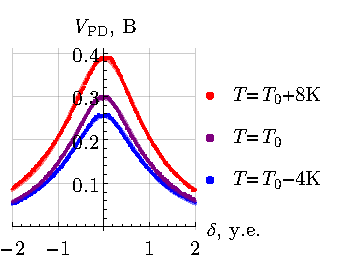
\includegraphics{figs/ovenD_v2.pdf}}
    \hspace{5 mm} 
    \subfigure[]{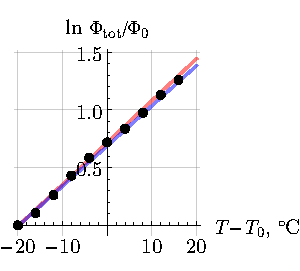
\includegraphics{figs/oven1_v4.pdf}}
    % \subfigure[]{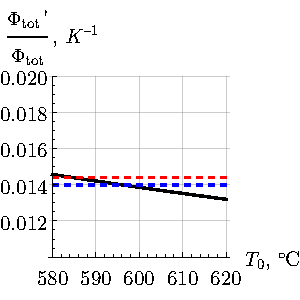
\includegraphics{figs/oven2_v4.pdf}}
    \subfigure[]{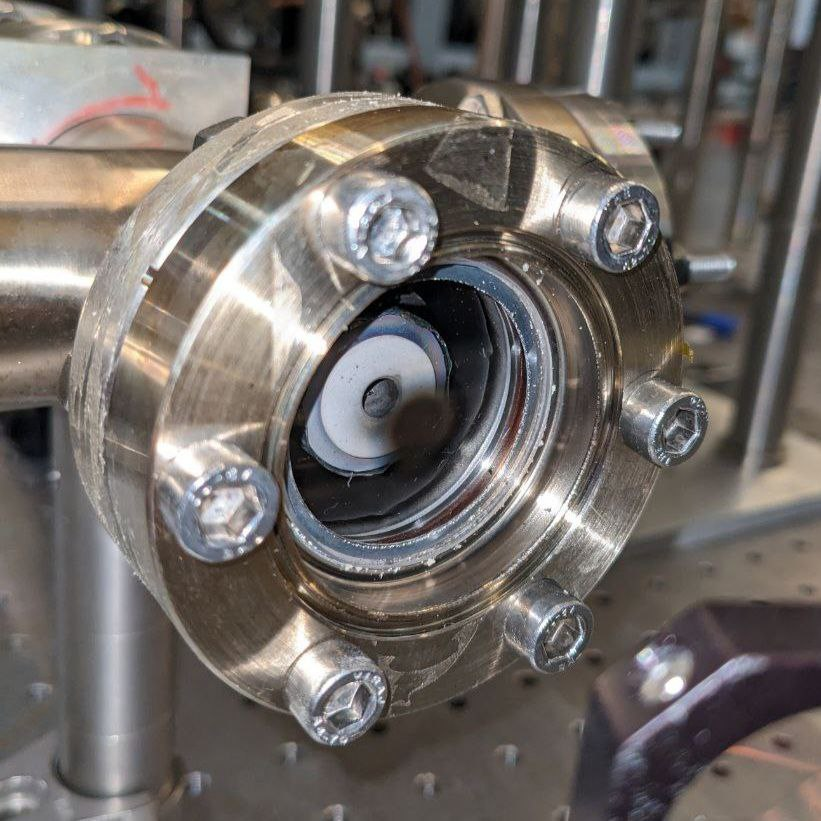
\includegraphics[width=0.25\textwidth]{figs/photo.jpg}}
    \vspace{-3mm}
    \caption{a) Снятая экспериментальная зависимость мощности флюоресценции атомарного пучка от величины отстройки от резонанса лазерного излучения. Непрерывным линиями показана аппроксимация данных лоренцовым контуром. б) Относительная зависимость потока атомов из печки $\sub{\Phi}{tot}$ от температуры: черными точками отмечены экспериментально снаятые точки, непрерывными линиями отмечены границы линейной апроксимации  в) Фотография напыленного на стекло алюминия при достижении температуры плавления}
    \label{fig:oven}
\end{figure}


Найдём логарифмическую производную $\sub{\Phi}{tot}'/\sub{\Phi}{tot}$, с помощью линейной аппроксимации зависимости $\ln \sub{\Phi}{tot} (T)/ \sub{\Phi}{0}$ (рис. \ref{fig:oven}б), где $\Phi_0 = \sub{\Phi}{tot}(T=T_0 - 20 \dC)$. Решая уравнение $\sub{n}{sat}'/\sub{n}{sat} = \sub{\Phi}{tot}'/\sub{\Phi}{tot} = \subt{V}{PD}' / \subt{V}{PD}$, находим  $T_0 = (590 \pm 10) \dC$.
% \red{(полученное значение согласуется с экспериментом по реперной точке на температуре плавления алюминия, стоит ли эту историю описывать?)}.

\upar{Определение температуры по реперной точке} 
Абсолютное значение температуры было проверено и другим способом. В тигель печи помещался кусочек алюминия, затем постепенно увеличивалась температура. При достижении температуры $T_0 + 65 \dC$ на окошко перед печью напылялся Al, что соответсвует температуре плавления $660 \dC$ и значению $T_0 = 595 \dC$, в соглавсовании с первым методом.

